\documentclass[a4paper, 11pt]{article}
\usepackage[utf8]{inputenc}
\usepackage{graphicx}
\usepackage{url}
\usepackage{hyperref}
\usepackage{color}
\usepackage{enumitem}

\title{LabSpace: A Collaborative Space where Knowledge and Experience is Shared}
\author{George E. Kallergis\\geokal@kth.se}
\date{\today{}}

\begin{document}

\maketitle

\begin{figure}[h!]
  \begin{center}
    
\includegraphics[width=\textwidth,height=\textheight,keepaspectratio]{imagery/logo.png}
    \label{fig:dneaf}
  \end{center}
\end{figure}

\textit{This document describes LabSpace, a collaborative space where students, professors, professionals and enthusiasts can exchange knowledge and experiences on a wide variety of areas including, but not limited to engineering, business, economics and art. The operational model and other implementation related details are discussed and analyzed to allow for an easy and quick adoption by any interested academic organization.}

\newpage

%========%
% Introduction %
%========%
% The introduction gives an overview of the vision and goals of LabSpace.
\section*{Introduction}
LabSpace is a specially engineered maker-space \cite{whatsamakerspace} targeting the academic environment where students, professors, professionals and other enthusiasts can meet and exchange theoretical and practical knowledge around a multitude of areas of interest (engineering, business, economics, art etc.). The main vision of LabSpace is the creation of a space where knowledge is shared in a borderless fashion. A place were students can enhance their knowledge and gain experience from  professionals, teachers or even other students. The desired outcome of this is educated individuals ready to undertake challenges met in the real world, covering  the interests of the students as well as the current needs of the market. Employment rates of young professionals, innovative start up companies as well as employing companies' satisfaction levels are all expected to increase as a long term result of a LabSpace implementation.


\section{Roles} \label{sec:roles}
Figure \ref{fig:ls_env} shows LabSpace inside its preferred context. Preferred context is defined as the ideal environment into which LabSpace is expected to acomplish it's goals in an efficient and sustainable manner.

\begin{figure}[h!]
  \begin{center}
    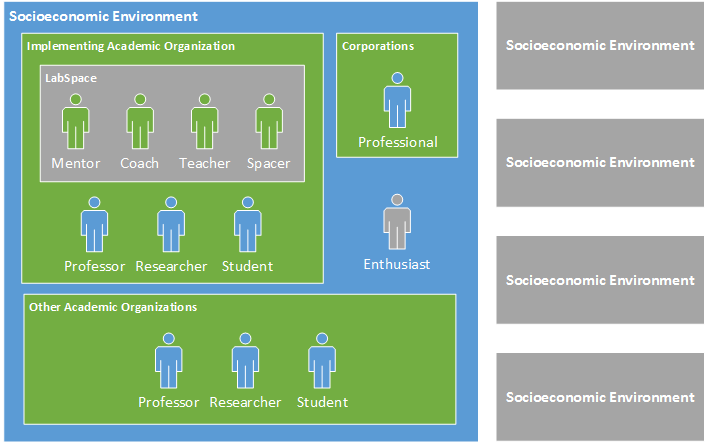
\includegraphics[width=350px,height=\textheight,keepaspectratio]{imagery/ls_context.png}
    \caption{LabSpace into the Preferred Context.}
    \label{fig:ls_env}
  \end{center}
\end{figure}

Each of the components is explained in more detail below:

\begin{itemize}[noitemsep]
    \item The \textit{implementing academic organization} is the academic organization (i.e. the university or school) that hosts LabSpace into its premises.
    \item The \textit{socioeconomic environment} is the society and the economy into which the \textit{implementing academic organization} operates in. In other words, this block models the country the \textit{implementing academic organization} is in, along with all of its social and financial forces that affect the operation of the latter.
    \item The \textit{corporations} denote the commercial organizations that are active in that particular \textit{socioeconomic environment}.
    \item The \textit{other academic organizations} block defines other universities or schools that although they are not implementing LabSpace, they contribute to an already existing implementation sharing people and other resources (see \ref{sec:bm_res}). The actors in Figure \ref{fig:ls_env} define the roles different people play in the different environments inside and outside of LabSpace. 
\end{itemize}

The different roles outside of LabSpace are defined as follows:

\begin{itemize}[noitemsep]
    \item \textit{Professor}. The person that is employed as a professor in either the \textit{implementing academic organization} or any \textit{other academic organization}.
    \item \textit{Researcher}. The person that is employed as a researcher in either the \textit{implementing academic organization} or any \textit{other academic organization}.
    \item \textit{Student}. The person that is studying at either the \textit{implementing academic organization} or any \textit{other academic organization}.
    \item \textit{Professional}. The person that is or has been employed by one or more \textit{corporations} (see definition above) and is either representing his/her organization or is contributing to LabSpace as an individual.
    \item \textit{Enthusiast}. The person that belongs to none of the above categories, but still contributes to LabSpace either by providing resources (see \ref{sec:bm_res}) or by taking part in different activities  (see \ref{sec:bm_activities}).
\end{itemize}

All of the above roles when active inside of LabSpace, turn into one (or multiple) of the following:

\begin{itemize}[noitemsep]
    \item \textit{Spacer}. The person that is learning and enhancing his/her skills inside LabSpace by participating to projects or being mentored, coached or teached by others.
    \item \textit{Mentor}. The person that is mentoring one or more spacers inside of LabSpace.
    \item \textit{Coach}. The person that is coaching one or more spacers inside of LabSpace.
    \item \textit{Teacher}. The person that is teaching one or more spacers inside of LabSpace.
\end{itemize}

Note here that multiple roles can be held by the same person inside of LabSpace. A person might be teaching someone, but at the same time being coached by someone else.

Observing LabSpace from a different perspective, we could see it as a transformation of roles. Inside of LabSpace it doesn't matter if you are a professor or a student, both can teach and both should be open to learning from anybody regardless of the roles they posses outside of LabSpace. It is a neutral zone from the knowledge perspective. The additional \textit{socioeconomic environment} blocks (right hand side of Figure \ref{fig:ls_env}) define the ability of a LabSpace to cooperate on a worldwide scale regardless of the country into which the \textit{implementing academic organization} operates in.


%\begin{quote}
%    \textit{""}
%\end{quote}


%=======%
% Operation %
%=======%
% The operation section discusses the operational model of LabSpace and how an interested academic organization can go about implementing it.
\section{Operation}

The operational model defines the way the described roles interact inside of LabSpace in order to promote its vision and accomplish its goals while sustaining the smooth operation of the space.

\subsection{LabSpace Operational Model}

Treating LabSpace as a business itself, we can model its operational model using the notion of a business model. This section specifies the following aspects of LabSpace:

\begin{itemize}[noitemsep]
    \item The different stakeholders of LabSpace.
    \item The channels required to reach each stakeholder from a marketing standpoint.
    \item The relationships build between LabSpace and each of the stakeholders.
    \item The unique value proposition offered by LabSpace.
    \item The key activities necessary for normal operation.
    \item The key resources necessary for normal operation.
    \item The costs incurred by the operation of LabSpace.
    \item The revenue streams that exist as a result of the operation of LabSpace.
\end{itemize}

Since LabSpace is an open specification released under a Creative Commons license, any interested organization can proceed with its implementation without requiring any kind of special permission whatsoever. The \textit{implementing academic organizations} can be located anywhere in the world and the resources available to them are expected to vary significantly. For this reason, in the following sections we avoid setting hard limitations on areas characterized by high variability (i.e. available equipment) and we mainly attempt to give a basic outline of "good to have" instead of "must have" features.

\subsubsection{The Stakeholders}

Stakeholders are the organizations or individuals that are immediately affected by the implementation of LabSpace and its operation. This section defines the responsibilities of each stakeholder in the LabSpace realm. Looking at Figure \ref{fig:ls_env} we can identify the stakeholders as follows:

\begin{itemize}[noitemsep]
    \item The \textit{implementing academic organizations}.
    \item The \textit{students}.
    \item The \textit{professors}.
    \item The \textit{researchers}.
    \item The \textit{enthusiasts}.
    \item The \textit{professionals}.
    \item The \textit{corporations}.
    \item The \textit{socioeconomic environment}.
\end{itemize}

The \textit{implementing academic organizations} are affected by a LabSpace implementation in a number of different ways. First and foremost, they provide hosting for a particular implementation in terms of housing and other utility resources such as electricity. Access to the premises of LabSpace is granted by the \textit{implementing academic organization} based on the rules already in effect. Different \textit{implementing academic organizations} have different rules when it comes to accessing their premises so, a LabSpace implementation should always abide to the existing rules to ensure minimal disruption of the current operational state of the hosting academic organization. Secondly, the \textit{implementing academic organization} acts as a provider of key resources (see \ref{sec:bm_res}) whether it is material resources or human resources. Finally, possible integration of LabSpace with courses provided by the \textit{implementing academic organization} and research programs undertaken by it is also something that falls under the responsibilities of the \textit{implementing academic organization}.

The \textit{students} are the ones that have the responsibility of implementing and executing LabSpace. The viability of the space is tightly dependent on the motivation and enthusiasm shown by the students. After all, the whole idea of LabSpace is geared towards the professional and personal development of students. Most of the key activities required for the smooth operation of LabSpace (see \ref{sec:bm_activities}) are mainly carried out by the \textit{students} although cooperation with other stakeholders is always encouraged and sometimes required (e.g. when decisions have to be made that collide with already existing rules by the hosting organizations). Taking into account the borderless knowledge exchange scheme that lives at the heart of LabSpace, \textit{students} can also act as teachers, coaches and mentors to others. Finally, they can also act as providers of key resources (see \ref{sec:bm_res}) if they so desire.

The \textit{professors} are the ones that are expected to teach, coach and mentor the most inside of LabSpace. In the case of course and research program integrations the initial steps have to be taken by the \textit{professors} and accepted by the \textit{implementing academic organization} according to the rules currently in effect. \textit{Professors} can also act as providers of key resources (see \ref{sec:bm_res}) if they so desire.

The \textit{researchers}, \textit{enthusiasts} and \textit{professionals} are also expected to teach, coach and mentor inside of LabSpace bringing in theoretical and practical experience that will help toward the development of \textit{spacers}. Similarly, they could also act as providers of key resources (see \ref{sec:bm_res}) if they so desire.

The \textit{corporations} are expected to bring the state of the art of their respective market into LabSpace. Real world projects can be brought in LabSpace giving everyone the chance to work on them and gain useful practical experience. The \textit{corporations} can be active in a LabSpace implementation through \textit{professionals} they employ or through \textit{professors} (or \textit{reearchers}) they cooperate with. Of course, they could also act as providers of key resources (see \ref{sec:bm_res}) if they so desire.

Finally, the \textit{socioeconomic environment} into which LabSpace is active can prove of high importance acting as a provider of resources (i.e. material or monetary) or as a means of raising awareness and promoting the LabSpace idea in an attempt to engage the different stakeholders already mentioned.

Figure \ref{fig:ls_responsibilities} summarizes all of the above.

\begin{figure}[h!]
  \begin{center}
    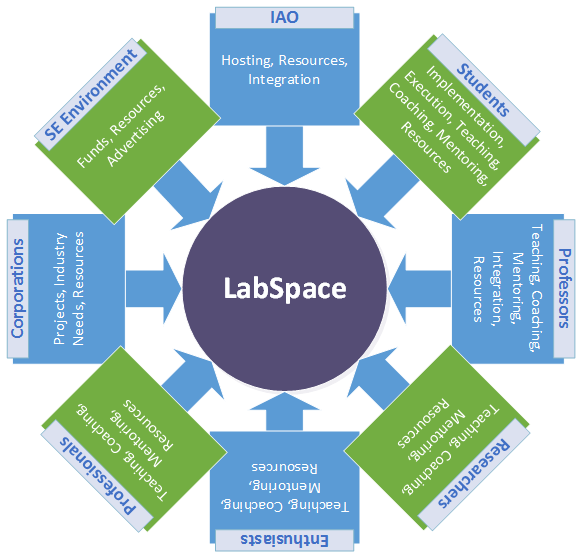
\includegraphics[width=285px,height=\textheight,keepaspectratio]{imagery/ls_stakeholders.png}
    \caption{Stakeholders' Responsibilities.}
    \label{fig:ls_responsibilities}
  \end{center}
\end{figure}


\subsubsection{The Channels}

\subsubsection{The Relationships}

\subsubsection{The Value Proposition}

\subsubsection{The Key Activities} \label{sec:bm_activities}
Resourse sharing.

\subsubsection{The Key Resources} \label{sec:bm_res}

\subsubsection{The Cost Structure}

\subsubsection{The Revenue Streams}


\subsection{Space Management}
\textit{The "fair use" policy will be defined here to ensure that the space can be used by anyone, but also specific resources can be bound for future use (e.g. breadboards and components to avoid assembly and disassembly of the circuit on every visit). Access to the building will be discussed here.}

\newpage

\begin{thebibliography}{9}
    \bibitem{whatsamakerspace} \emph{What’s a Makerspace?} (n.d.) [Online]. Available: \\ \href{http://makerspace.com/home-page}{http://makerspace.com/home-page} (Accessed: February 3\textsuperscript{rd}, 2014).
\end{thebibliography}

\end{document}
